\documentclass[10pt]{article}
\usepackage[utf8]{inputenc}

\usepackage{graphicx}
\usepackage{amsmath}
\usepackage{amsfonts}
\usepackage{mathtools}
\usepackage{siunitx}
\usepackage{braket}
\usepackage{parskip}
\usepackage{wrapfig}

\usepackage[letterpaper, portrait, margin=1in]{geometry}
\renewcommand{\baselinestretch}{1.1}

\title{Quantum HW4}
\author{bellenchia}
\date{February 2019}
\begin{document}
\maketitle




\section*{11.) Projection onto a Basis}
\subsection*{11a, 11b, 11c}
We are given the wavefunction $\psi(x)=\frac{1}{\sqrt{L}}[\frac{1}{4}-(\frac{x}{L}-\frac{1}{2})^2]$\\

Using bra-ket representation for $\psi(x)=\sum_{n=1}^\infty c_nf_n(x)$ where $c_n={\displaystyle\int_0^L}f_x(x)^*\psi(x)dx$\\
We get $\psi(x)=\sum_{n=1}^\infty c_n\ket{f_n}$ where  $c_n=\braket{f_n|\psi}$\\

%\subsection*{11b}
Solving the integral $c_n={\displaystyle\int_0^L}f_x(x)^*\psi(x)dx=\frac{1}{\sqrt{L}}{\displaystyle\int_0^L}(\frac{x}{L}-\frac{x^2}{L^2})sin(\frac{n\pi x}{L})dx$\\

We get $c_n=\frac{2\sqrt{L}}{\pi^3}\frac{1-(-1)^n}{n^3}$. Thus, $c_1=\frac{4\sqrt{L}}{\pi^3}$, $c_2=0$, $c_3=\frac{4\sqrt{L}}{27\pi^3}$, $c_4=0$\\
%\subsection*{11c}
\begin{center}
    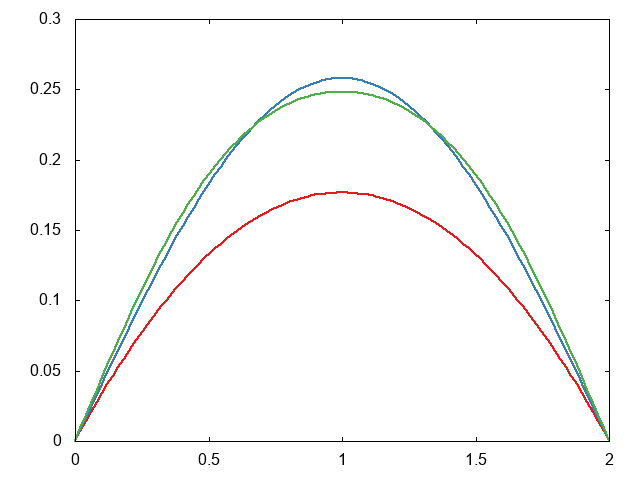
\includegraphics[width=0.6\linewidth]{q11_7.png}\\
Above is our plot for $\psi(x)$, along with $\sum_{i=1}^{n}c_nf_n$ for $n=2$, $n=4$\\
\end{center}

\pagebreak

\section*{12.) Commutator Push-ups}
For the following commutators, we use $[\hat{A},\hat{B}]=\hat{A}\hat{B}-\hat{B}\hat{A}$\\
\subsection*{12a}
$[\hat{\frac{1}{x}},\hat{p}_x]=\frac{-i\hbar}{x}\frac{df}{dx}+i\hbar\frac{d}{dx}(\frac{1}{x}f)$\\
$=\frac{-i\hbar}{x}\frac{df}{dx}+[\frac{-1}{x^2}f+\frac{1}{x}\frac{df}{dx}]$\\
$=\frac{\hbar}{ix^2}$\\
\subsection*{12b}
$[V(x),\hat{p}_x]=-i\hbar V(x)\frac{df}{dx}+[V'(x)f(x)+V(x)\frac{df}{dx}=i\hbar V'(x)$ Where $V'(x)=\frac{dV}{dx}$\\
\subsection*{12c}
Since we know ;
\[
\hat{i}\hat{j}=\delta_{ij}=
\begin{cases}
1 & i=j\\
0 & i\neq j
\end{cases}
\]
\\
We multiply the polynomials and find;\\

$[\hat{x}\hat{p}_y-\hat{y}\hat{p_x},\hat{y}\hat{p}_z-\hat{z}\hat{p}_y]=-\hat{p}_x\hat{p}_z+\hat{p}_z\hat{p}_x$\\

$=-i\hbar\frac{d}{dx}(-i\hbar\frac{d}{dz})+i\hbar\frac{d}{dz}(-i\hbar\frac{d}{dx})$\\
\subsection*{12d}
For simplicity, we will use $\frac{d}{dx}=\partial_x$, $\frac{d}{dx}\frac{d}{dy}=\partial_{xy}$, etc.\\

$[x^2\frac{d^2}{dy^2},y\frac{d}{dx}]=x^2\partial_y(\partial_xf+y\partial{yx}f)-y\partial_x(x^2\partial{yy}f)$\\

$=x^2(\partial_{yx}f+\partial_{yx}f+y\partial_{yyx}f-2xy\partial_{yy}f-x^2y\partial_{xyy}f$\\

$\Rightarrow[x^2\frac{d^2}{dy^2},y\frac{d}{dx}]=x^2y(\frac{d^2}{dy^2}\frac{d}{dx}-\frac{d}{dx}\frac{d^2}{dy^2})+2(x^2\frac{d}{dy}\frac{d}{dx}-xy\frac{d^2}{dy}^2)$\\

\section*{13.) Vector Spaces}
Let me brush off my Abstract Algebra textbook and we'll get down to business;
\subsection*{13a}
We must show the set $A$ exhibits all properties of a vector space, $A=\{p_i(x)\in\mathbb{C}_n[x]$ s.t. $p_i(1)=0\}$\\

$A\subset\mathbb{C}_n[x]=\{p_k(x)=c_0+c_1x+c_2x^2+...+c_kx^n|c_i\in\mathbb{C},0\leq k\leq n<N\}$\\

$u+v=v+u$\\
$u+(v+w)=(u+v)+w$\\
$\exists 0\in V s.t. \forall v\in V v+0=v$\\
$\forall v\in V, \exists(-v) s.t. v+(-v)=0$\\

These conditions hold because our set A is a subset of the Abelian group $\mathbb{C}_n[x]$, and because $p_i(1)=0$. If this was not the case, and instead $p_i(1)=k$, $k\in\mathbb{C}$, we would have
$p_j(1)=p_i(1)+p_j(1)=2k\Rightarrow p_j(x)\not\in A$\\

For the rest of this we will assume $p_n,p_m\in A$ are two polynomials of degree n, m respectively.\\
$(a+b)p_n(x)=ap_n(x)+bp_n(x)$, this is trivial.\\
$c(dp_n(x))=(cd)p_n(x)$, also given since $\mathbb{C}$ is Abelian.\\

Finally, $\exists 1\in A$ $s.t. 1p_m(x)=p_m(x)$  $\forall p_m(x)\in A$ of course this element is simply 1.\\

Having verified all the necessary properties, the aforementioned set is indeed a vector space.\\

\subsection*{13b}

We know for a finite dimensional vector space the \textbf{trace}, (the sum of terms along the diagonal) is equal to the dimension of the vector space for the identity operator;\\

$Trace(\hat{I})=n$\\

For purpose of proof by contradiction, let us assume $[\hat{A},\hat{B}]=\hat{I}$\\
Then we should have $Trace(AB-BA)=Trace(I)$\\
$\Leftrightarrow Trace(AB)-Trace(BA)=Trace(I)$\\
Since a property of the Trace is $Trace(AB)=Trace(BA)$, we see we get; \\
$Trace(AB)-Trace(AB)=n$\\
$0=n$\\

Thus, we have reached a contradiction, and it is impossible for $[\hat{A},\hat{B}]=\hat{I}$\\
\pagebreak
\section*{14.) Commuting Observables and Quantum Numbers}
\subsection*{14a}
To show any linear combination of the latter two basis vectors also has the eigenvalue $E_2$;\\

$\hat{H}(c_1\ket{\beta}+c_2\ket{\gamma})=c_1\hat{H}\ket{\beta}+c_2\hat{H}\ket{\gamma}=E_2\hat{H}(c_1\ket{\beta}+c_2\ket{\gamma})$\\
\subsection*{14b}
Representing the operator $\hat{H}$ as a matrix is extremely straighforward;\\

$\begin{bmatrix}
E_1 & 0 & 0 \\
 0 & E_2 & 0 \\
 0 & 0 & E_2
\end{bmatrix}$
\subsection*{14c}
We find our Matrix for $\hat{A}$ and evaluate $\hat{H}\cdot\hat{A}$;\\

$\begin{bmatrix}
 E_1 & 0 & 0 \\
 0 & E_2 & 0 \\
 0 & 0 & E_2
\end{bmatrix}
\cdot
\begin{bmatrix}
a & 0 & 0 \\
0 & b & ic \\
0 & -ic & b
\end{bmatrix}
=
\begin{bmatrix}
aE_1 & 0 & 0\\
0 & bE_2 & icE_2\\
0 & -icE_2 & bE_2
\end{bmatrix}$\\

Now, to show $\hat{A}$ and $\hat{H}$ commute;\\

$\hat{H}\cdot\hat{A}=
\begin{bmatrix}
a & 0 & 0 \\
0 & b & ic \\
0 & -ic & b
\end{bmatrix}
\cdot
\begin{bmatrix}
 E_1 & 0 & 0 \\
 0 & E_2 & 0 \\
 0 & 0 & E_2
\end{bmatrix}
=
\begin{bmatrix}
aE_1 & 0 & 0\\
0 & bE_2 & icE_2\\
0 & -icE_2 & bE_2
\end{bmatrix}$\\
\subsection*{14d}
Clearly, the eigenvalues of $\hat{H}$ are $\lambda_H=E_1$, $E_2$, and we can find $\lambda_A$ by solving the characteristic equation, ;\\

[$\hat{A}-\lambda\hat{I}]=0\Rightarrow(a-\lambda)(b-\lambda)^2-(\lambda-a)(ic)^2\Leftrightarrow\lambda^2-2b\lambda+(b^2-c^2)=0$\\

Immediately we see $\lambda=a$ is a solution, for the others we use the quadratic formula;  $\lambda=\frac{(2b)\pm\sqrt{4b^2-4(b^2-c^2)}}{2}$\\

$\Rightarrow \lambda_A=b\pm c$\\

Thus, the simultaneous Eigenkets are $\ket{\lambda_H,\lambda_A}=\ket{E_1,a},\ket{E_2,b+c}$, $\ket{E_2,b-c}$\\
\pagebreak
\section*{15.) Ehrenfest's Theorem}

The rate of change of the expectation value is given by the \textbf{Energy-Time Uncertainty Principle};\\

$\frac{d\langle p\rangle}{dt}=\frac{i}{\hbar}\langle[\hat{H},\hat{p}]\rangle+\langle\frac{d\hat{p}}{dt}\rangle$\\

evaluating the commutator $[\hat{H},\hat{p}]$, we get;

$[\hat{H},\hat{p}]=[\frac{p^2}{2m}+V(x),\hat{p}]$;\\

Since $\hat{p}$ commutes with itself, we know $[\hat{H},\hat{p}]=[V(x),\hat{p}]$ which we solved for in \textbf{12b}\\

$\frac{d\langle p\rangle}{dt}=\frac{i}{\hbar}\langle i\hbar\frac{dV}{dx}\rangle+\langle\frac{d\hat{p}}{dt}\rangle$\\

Additionally, since $\hat{p}$ does not depend explicitly on time, we know;\\

$\langle\frac{d\hat{p}}{dt}\rangle=0$, which simplifies our answer to $\frac{d\langle p\rangle}{dt}=\frac{i}{\hbar}\langle i\hbar\frac{dV}{dx}\rangle=-\langle\frac{dV}{dx}\rangle$\\

Thus, we have proven the desired relation;\\

\huge{$\frac{d\langle p\rangle}{dt}=-\langle\frac{dV}{dx}\rangle$}\\

\end{document}
